% Created 2022-02-24 Thu 08:00
% Intended LaTeX compiler: pdflatex
\documentclass[presentation,aspectratio=169]{beamer}
\usepackage[utf8]{inputenc}
\usepackage[T1]{fontenc}
\usepackage{graphicx}
\usepackage{grffile}
\usepackage{longtable}
\usepackage{wrapfig}
\usepackage{rotating}
\usepackage[normalem]{ulem}
\usepackage{amsmath}
\usepackage{textcomp}
\usepackage{amssymb}
\usepackage{capt-of}
\usepackage{hyperref}
\usepackage{khpreamble}
\usepackage{amssymb}
\usepgfplotslibrary{groupplots}
\usepackage{gensymb}
\newcommand*{\shift}{\operatorname{q}}
\usetheme{default}
\author{Kjartan Halvorsen}
\date{\today}
\title{Incremental encoder}
\hypersetup{
 pdfauthor={Kjartan Halvorsen},
 pdftitle={Incremental encoder},
 pdfkeywords={},
 pdfsubject={},
 pdfcreator={Emacs 26.3 (Org mode 9.4.6)}, 
 pdflang={English}}
\begin{document}

\maketitle

\section{Sensors in general}
\label{sec:orgfbe3441}
\begin{frame}[label={sec:orgdc68ec9}]{Sensors}
\begin{center}
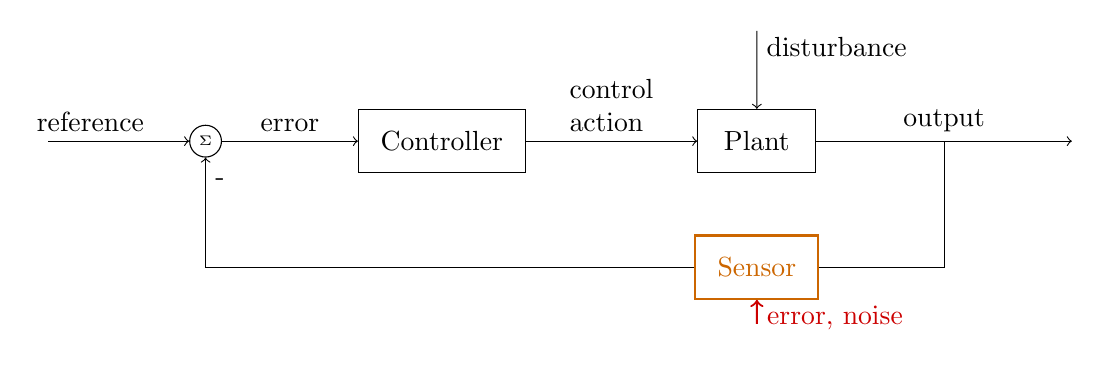
\begin{tikzpicture}[scale=0.6, node distance=22mm, block/.style={rectangle, draw, minimum width=15mm, inner sep=8pt}, sumnode/.style={circle, draw, inner sep=2pt}]

  \node[coordinate] (input) {};
  \node[sumnode, right of=input, node distance=20mm] (sumerr) {\tiny $\Sigma$};
  \node[block, right of=sumerr, node distance=30mm] (fb)  {Controller};
  \node[block, right of=fb, node distance=40mm] (plant)  {Plant};
  \node[block, orange!80!black, thick, below of=plant, node distance=16mm] (sensor)  {Sensor};

  \node[coordinate, above of=plant, node distance=14mm] (disturbance) {};
  \node[coordinate, right of=plant, node distance=40mm] (output) {};

  \draw[->] (input) -- node[above, pos=0.3] {reference} (sumerr);
  \draw[->] (sumerr) -- node[above] {error} (fb);
  \draw[->] (fb) -- node[above, align=left,] {control\\action} (plant);
  \draw[->] (plant) -- node[coordinate] (meas) {} node[above,] {output} (output);
  \draw[->] (disturbance) -- node[right, pos=0.2] {disturbance} (plant);
  \draw[->] (meas) |- (sensor) -| node[right, pos=0.9] {-} (sumerr);
  \draw[->, red!80!black, thick] (sensor) ++(0, -12mm) -- node[near start, right] {error, noise} (sensor);
  \end{tikzpicture}
\end{center}

\pause
It is \alert{inevitable} that sensors introduce \alert{noise} into the system.
\end{frame}

\begin{frame}[label={sec:orgb627ee2}]{Sensors}
\begin{center}
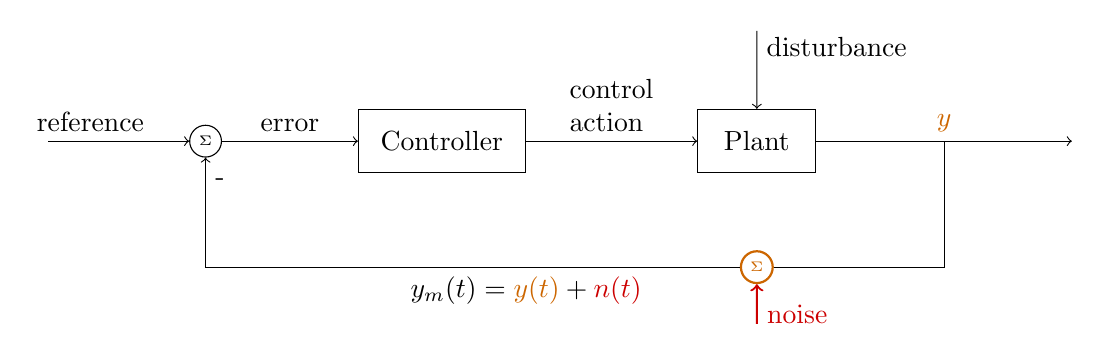
\begin{tikzpicture}[scale=0.6, node distance=22mm, block/.style={rectangle, draw, minimum width=15mm, inner sep=8pt}, sumnode/.style={circle, draw, inner sep=2pt}]

  \node[coordinate] (input) {};
  \node[sumnode, right of=input, node distance=20mm] (sumerr) {\tiny $\Sigma$};
  \node[block, right of=sumerr, node distance=30mm] (fb)  {Controller};
  \node[block, right of=fb, node distance=40mm] (plant)  {Plant};
  \node[sumnode, orange!80!black, thick, below of=plant, node distance=16mm] (sensor)  {\tiny $\Sigma$};


  \node[coordinate, above of=plant, node distance=14mm] (disturbance) {};
  \node[coordinate, right of=plant, node distance=40mm] (output) {};

  \draw[->] (input) -- node[above, pos=0.3] {reference} (sumerr);
  \draw[->] (sumerr) -- node[above] {error} (fb);
  \draw[->] (fb) -- node[above, align=left,] {control \\action} (plant);
  \draw[->] (plant) -- node[coordinate] (meas) {} node[above, orange!80!black] {$y$} (output);
  \draw[->] (disturbance) -- node[right, pos=0.2] {disturbance} (plant);
  \draw[->] (meas) |- (sensor) -| node[pos = 0.2, below] {$y_m(t) = \textcolor{orange!80!black}{y(t)} + \textcolor{red!80!black}{n(t)}$} node[right, pos=0.9] {-} (sumerr);
  \draw[->, red!80!black, thick] (sensor) ++(0, -12mm) -- node[near start, right] {noise} (sensor);
  \end{tikzpicture}
\end{center}

It is important to know the (statistical) characteristics of the measurement error!

 \begin{center}
 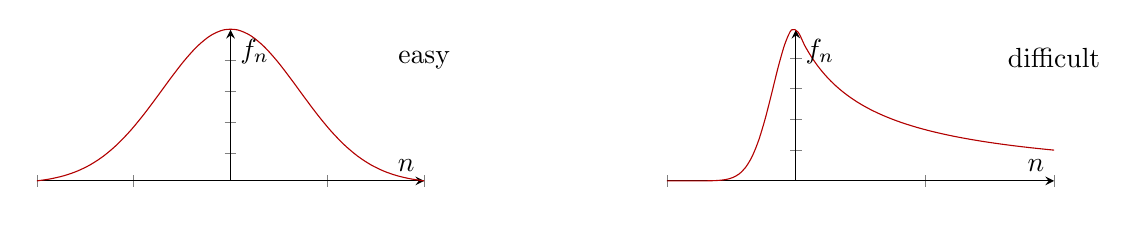
\begin{tikzpicture}
   \begin{axis}[clip=false,width=6.5cm, height=3.5cm, xticklabel=\empty, yticklabel=\empty,
   axis lines=middle,
   ylabel={$f_n$}, xlabel={$n$}]
   \addplot[red!70!black, no marks, smooth, domain=-2:2, samples=30] {exp(-pow(x,2))};
   \node at (axis cs: 2,0.8) {easy};
   \end{axis}
%   \begin{axis}[clip=false, xshift=5cm, width=4.5cm, height=3.5cm, xticklabel=\empty, yticklabel=\empty,
%   axis lines=middle,
%   ylabel={$f_n$}, xlabel={$n$}]
%   \addplot[red!70!black, no marks, smooth, domain=-4:6, samples=60] {exp(-pow((x-2)*2,2)) + exp(-pow((x+0.5)*2,2)) };
%   \node at (axis cs: 4,0.8) {difficult};
%   \end{axis}
   \begin{axis}[clip=false, xshift=8cm, width=6.5cm, height=3.5cm, xticklabel=\empty, yticklabel=\empty,
   axis lines=middle,
   ylabel={$f_n$}, xlabel={$n$}]
   \addplot[red!70!black, no marks, smooth, domain=-2:4, samples=60] {(x<0)*exp(-pow((x)*2,2)) + (x>=0)/(1+x) };
   \node at (axis cs: 4,0.8) {difficult};
   \end{axis}
 \end{tikzpicture}
 \end{center}
\end{frame}


\begin{frame}[label={sec:org193c061}]{Sensors - characteristics}
\begin{columns}
\begin{column}{0.4\columnwidth}
\begin{itemize}
\item \alert{Accuracy} How correct is the measurement on average
\item \alert{Precision} How much do the errors vary (standard deviation)
\item \alert{Sensitivity/resolution} The smallest change in the measured variable that can be detected
\item \alert{Delay} \(y_m(t) = y(t-\tau) + n(t)\)
\item \alert{Sampling and digitalization}
\end{itemize}
\end{column}

\begin{column}{0.6\columnwidth}
\pause

\begin{center}
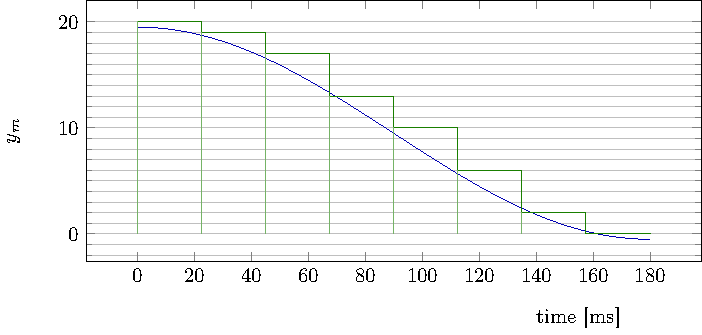
\includegraphics[width=0.96\textwidth]{../../figures/sampling-digitalization}
\end{center}
\end{column}
\end{columns}
\end{frame}

\section{Encoder}
\label{sec:org2dadea7}
\begin{frame}[label={sec:orgabf93e3}]{Incremental encoder}
\begin{center}
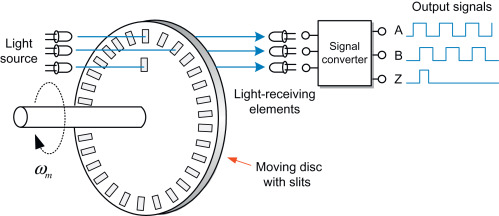
\includegraphics[width=0.7\textwidth]{../../figures/encoder-im.jpg}
{\tiny Source: \url{https://www.sciencedirect.com/topics/engineering/incremental-encoder}}
\end{center}
\end{frame}

\begin{frame}[label={sec:org5eeffed}]{Incremental encoder}
\begin{center}
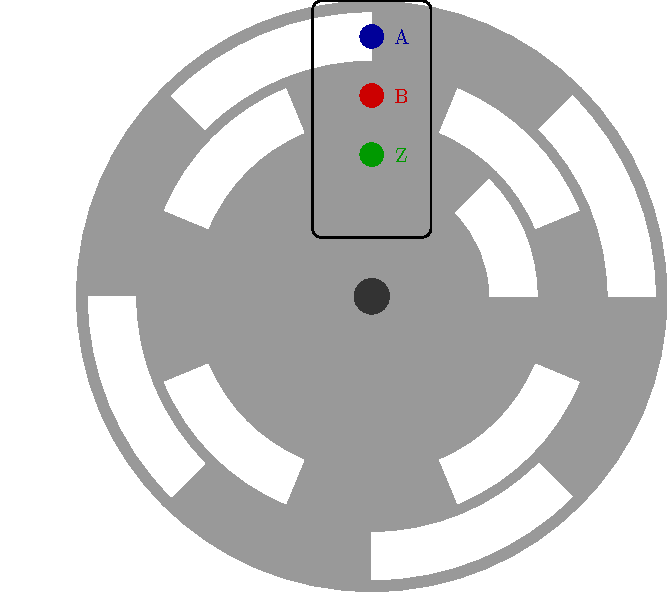
\includegraphics[width=0.4\textwidth]{../../figures/encoder-disc}
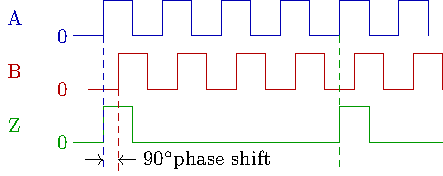
\includegraphics[width=0.5\textwidth]{../../figures/encoder-signals}
\end{center}

\emph{Pulses Per Revolution (PPR)} is 4 en the example. Each aperture covers a sector of \(\frac{360\degree}{2 \times PPR} = 45\degree\).
\end{frame}

\begin{frame}[label={sec:org3f531f4}]{Incremental encoder}
\begin{center}
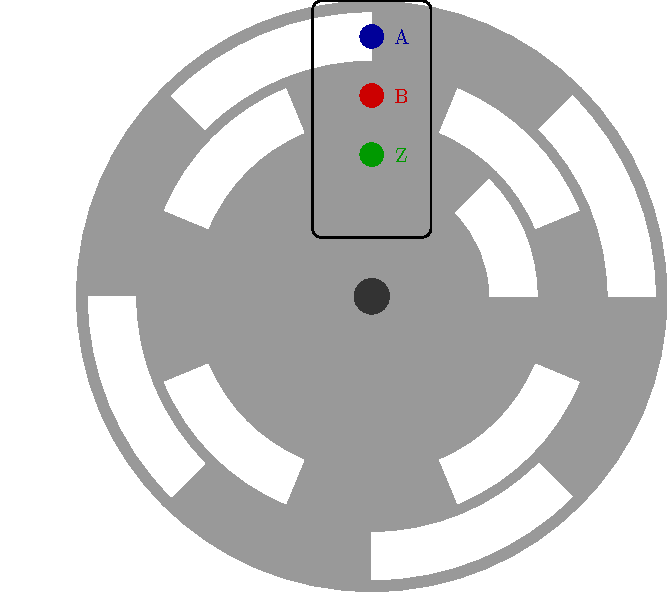
\includegraphics[width=0.4\textwidth]{../../figures/encoder-disc}
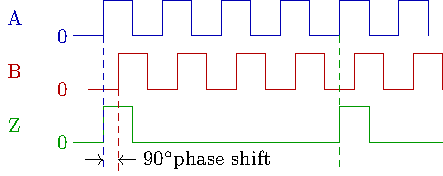
\includegraphics[width=0.5\textwidth]{../../figures/encoder-signals}
\end{center}

\alert{Activity} If both rising \alert{and} falling edges of both signals \textcolor{blue!80!black}{A} and \textcolor{red!80!black}{B}, what is the smallest change in angle that can be detected (\emph{sensitivity} of the sensor)?
\end{frame}


\begin{frame}[label={sec:org6511fde}]{Incremental encoder}
\begin{center}
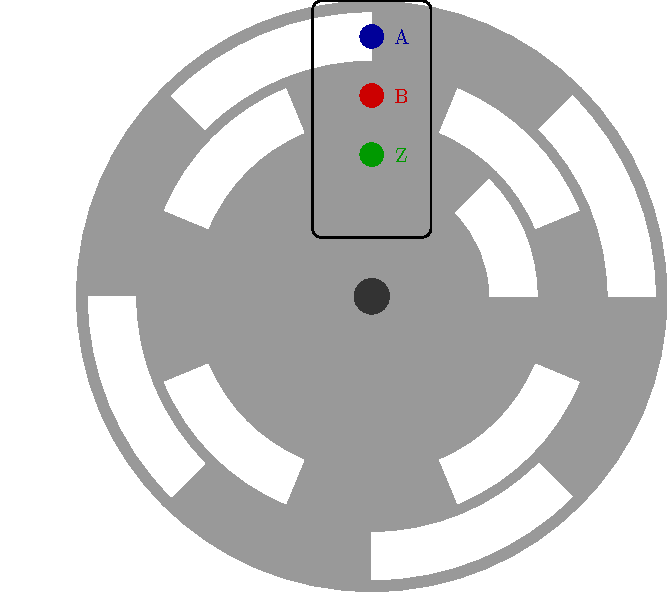
\includegraphics[width=0.4\textwidth]{../../figures/encoder-disc}
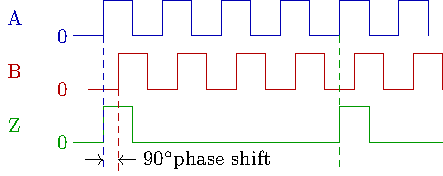
\includegraphics[width=0.5\textwidth]{../../figures/encoder-signals}
\end{center}

\alert{Activity} In the above example, does the encoder turn clockwise (CW) or counter-clockwise (CCW)?
\end{frame}


\begin{frame}[label={sec:org3daab96}]{Incremental encoder - velocity}
\begin{columns}
\begin{column}{0.5\columnwidth}
\begin{center}
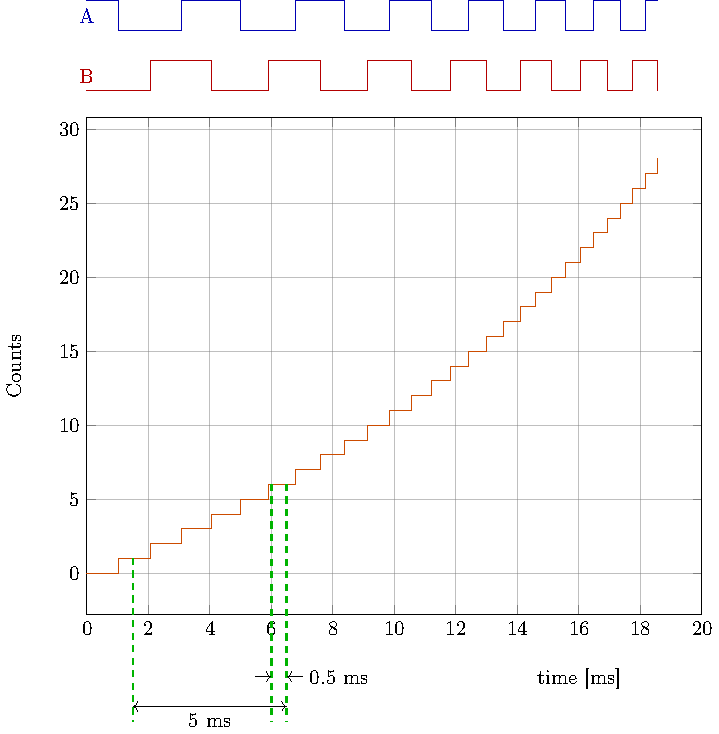
\includegraphics[width=\textwidth]{../../figures/encoder-signals-nonuniform}
\end{center}
\end{column}
\begin{column}{0.5\columnwidth}
We want to find the angular velocity at the time-instant \(t=\unit{6.5}{\milli\second}\). For the encoder we have PPR=8, and both rising and falling edges of both signals A and B are counted, resulting in 32 counts per revolution.

\alert{Activity} Calculate the angular velocity in rad/s for case \alert{(a)} using a sampling period of \(\Delta t=\unit{0.5}{\milli\second}\), and for case \alert{(b)} using a sampling period of \(\Delta t=\unit{5}{\milli\second}\).
\end{column}
\end{columns}
\end{frame}






\begin{frame}[label={sec:org6bd94a1}]{Incremental encoder - Velocity from frequency of the counts}
\begin{columns}
\begin{column}{0.5\columnwidth}
\begin{center}
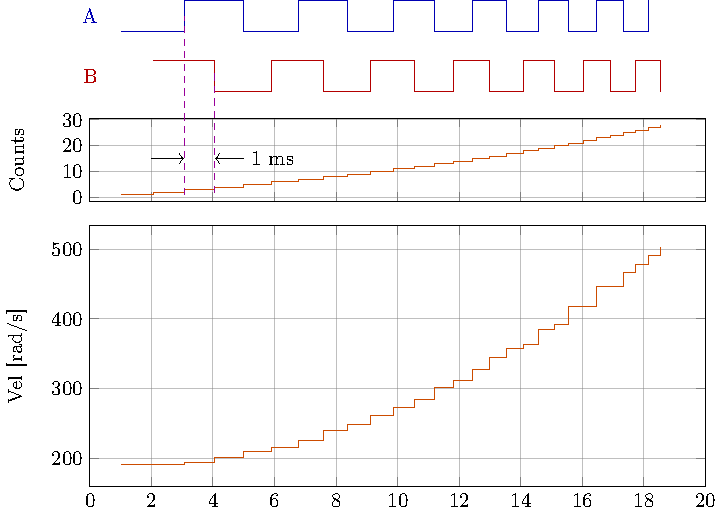
\includegraphics[width=\textwidth]{../../figures/encoder-signals-freqs}
\end{center}
\end{column}
\begin{column}{0.5\columnwidth}
The velocity can be measured by the inverse of the time between subsequent pulses. In the example there is an interval of \unit{1}{\milli\second} between the two pulses. The velocity becomes
\begin{align*}
 v &= 1 \, \text{pulses/ms} = \frac{1/32 \, \text{revolutions}}{\unit{10^{-3}}{\second}}\\
 &= \unit{\frac{2\pi}{32}\times 1000}{\rad\per\second} = \unit{196.3}{\rad\per\second}
 \end{align*}
\end{column}
\end{columns}
\end{frame}






\begin{frame}[label={sec:org7d3f8ed}]{Incremental encoder - Velocity from frequency of the counts}
\begin{columns}
\begin{column}{0.5\columnwidth}
\begin{center}
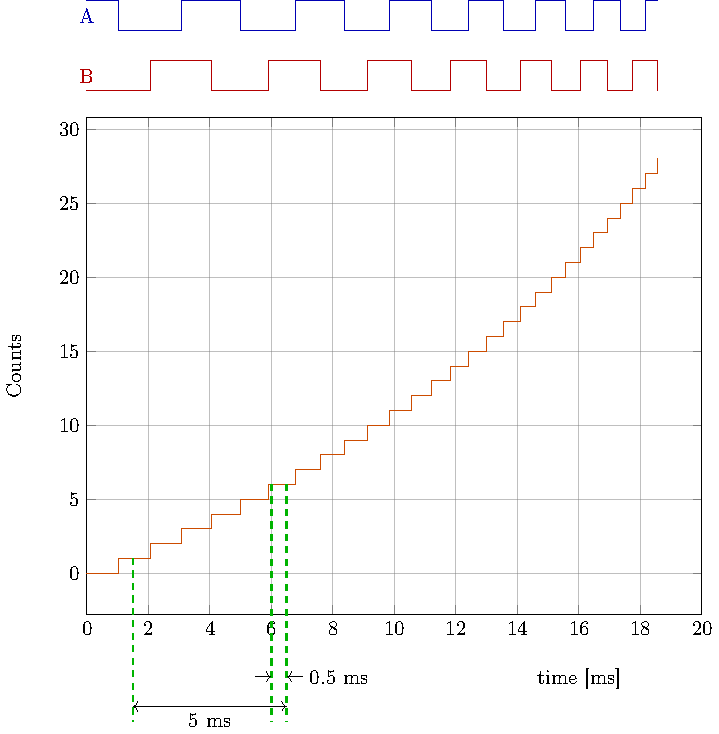
\includegraphics[width=\textwidth]{../../figures/encoder-signals-nonuniform}
\end{center}
\end{column}
\begin{column}{0.5\columnwidth}
\alert{Activity} Calculate the velocity!
\end{column}
\end{columns}
\end{frame}






\begin{frame}[label={sec:orgd750b5c}]{Simulink exercise - decoder}
Complete the simulink diagram so that the angular velocity is correctly estimated.

\begin{center}
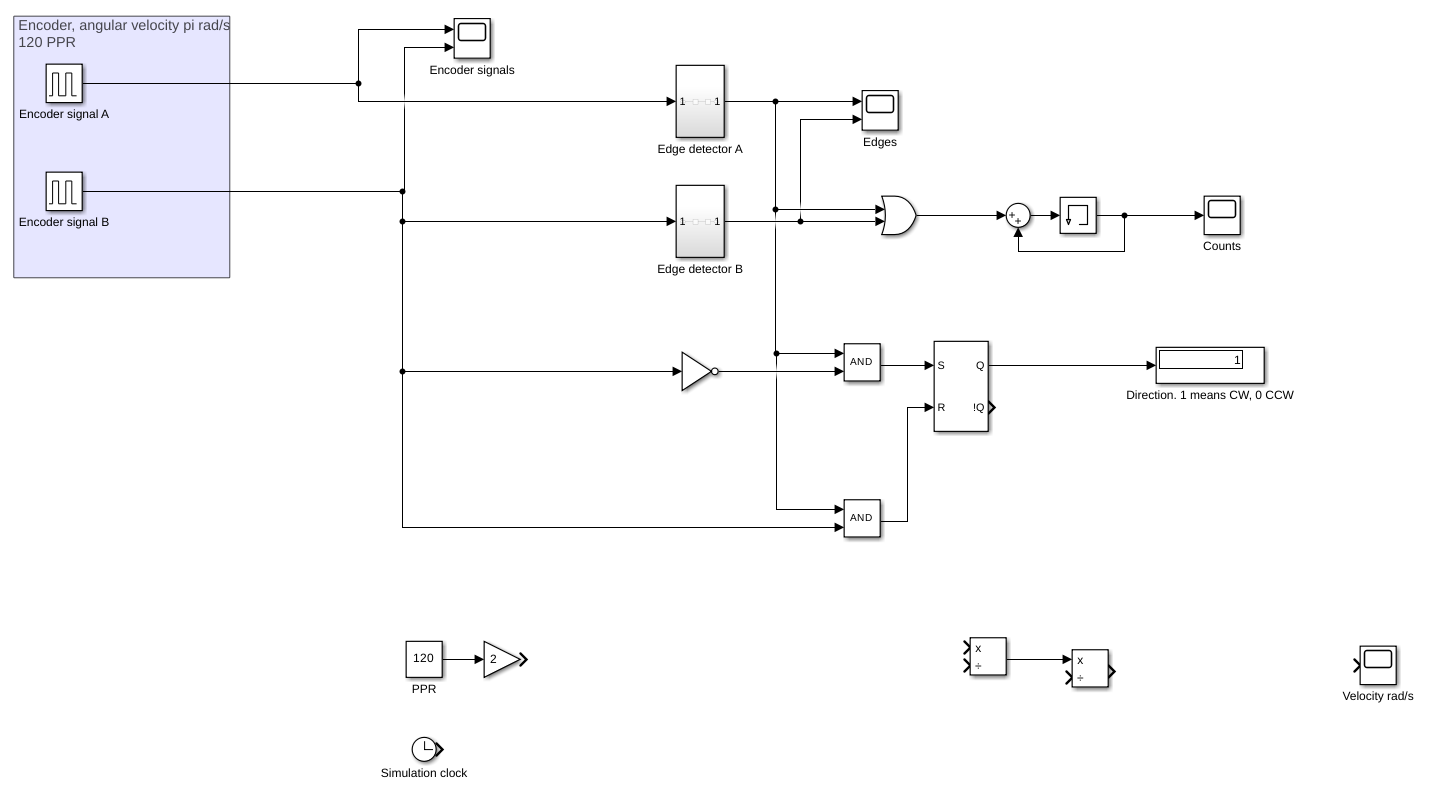
\includegraphics[width=0.8\textwidth]{../../figures/simulink-encoder-decoder-exc.png}
\end{center}
\end{frame}
\end{document}